\documentclass[11pt, letterpaper]{report}
\usepackage[utf8]{inputenc}
\usepackage[T1]{fontenc}
\usepackage{helvet}
\renewcommand{\familydefault}{\sfdefault}
\usepackage{graphicx}
\usepackage{lipsum}
\usepackage[top=1in, bottom=1in, left=1in, right=1in]{geometry}
\usepackage{fancyhdr}
\usepackage{tocloft}
\usepackage{caption}
\captionsetup[figure]{labelfont={bf},name={Figure},labelsep=period, font={it}}
\usepackage{xltabular}
\usepackage{titlesec}
\titleformat{\chapter}[hang] 
{\normalfont\huge\bfseries}{}{1em}{} 
\titlespacing*{\chapter}{0pt}{0pt}{40pt}

\begin{document}
% Cover page
\newgeometry{top=2in, bottom=2in, left=2in, right=2in}
\begin{titlepage}
    \centering
    
\includegraphics[width=\textwidth]{images/logo.png}\par
    \vspace{1cm}
    {\bfseries SE 463: Software Requirements: Specification \& Analysis: \par}
    \vspace{0.5cm}
    {Daniel Berry \par}
    \vspace{5cm}
    {Group 01: \par}
    {Nishesh Jagga \par}
    {20741914 \par}
    \vspace{5cm}
    {Friday, July 14, 2023 \par}
\end{titlepage}
\restoregeometry

% Table of Contents
\tableofcontents
\thispagestyle{empty}
\clearpage

% Custom header and footer
\pagestyle{fancy}
\fancyhf{}
\rfoot{\thepage}
\lfoot{Deliverable 4}
\renewcommand{\headrulewidth}{0pt}

% Abstract
\chapter{Abstract}
\setcounter{page}{1}
A tool that aids a user in maintaining their budget by scheduling their weekly meals through suggesting recipes sourced from an online recipe database, that are suitable for their budget and align with their dietary restrictions. Following a personalization process, the users can expect to be presented with recipes that they might like to eat, made using ingredients that fit their budget, with prices from their local grocery store. To aid the grocery shopping process, any missing ingredients for the recipes in their planned meals would be added to a grocery list for the user to follow while shopping.

% Domain Model
\chapter{Domain Model}
\begin{figure}[h]
    \centering
    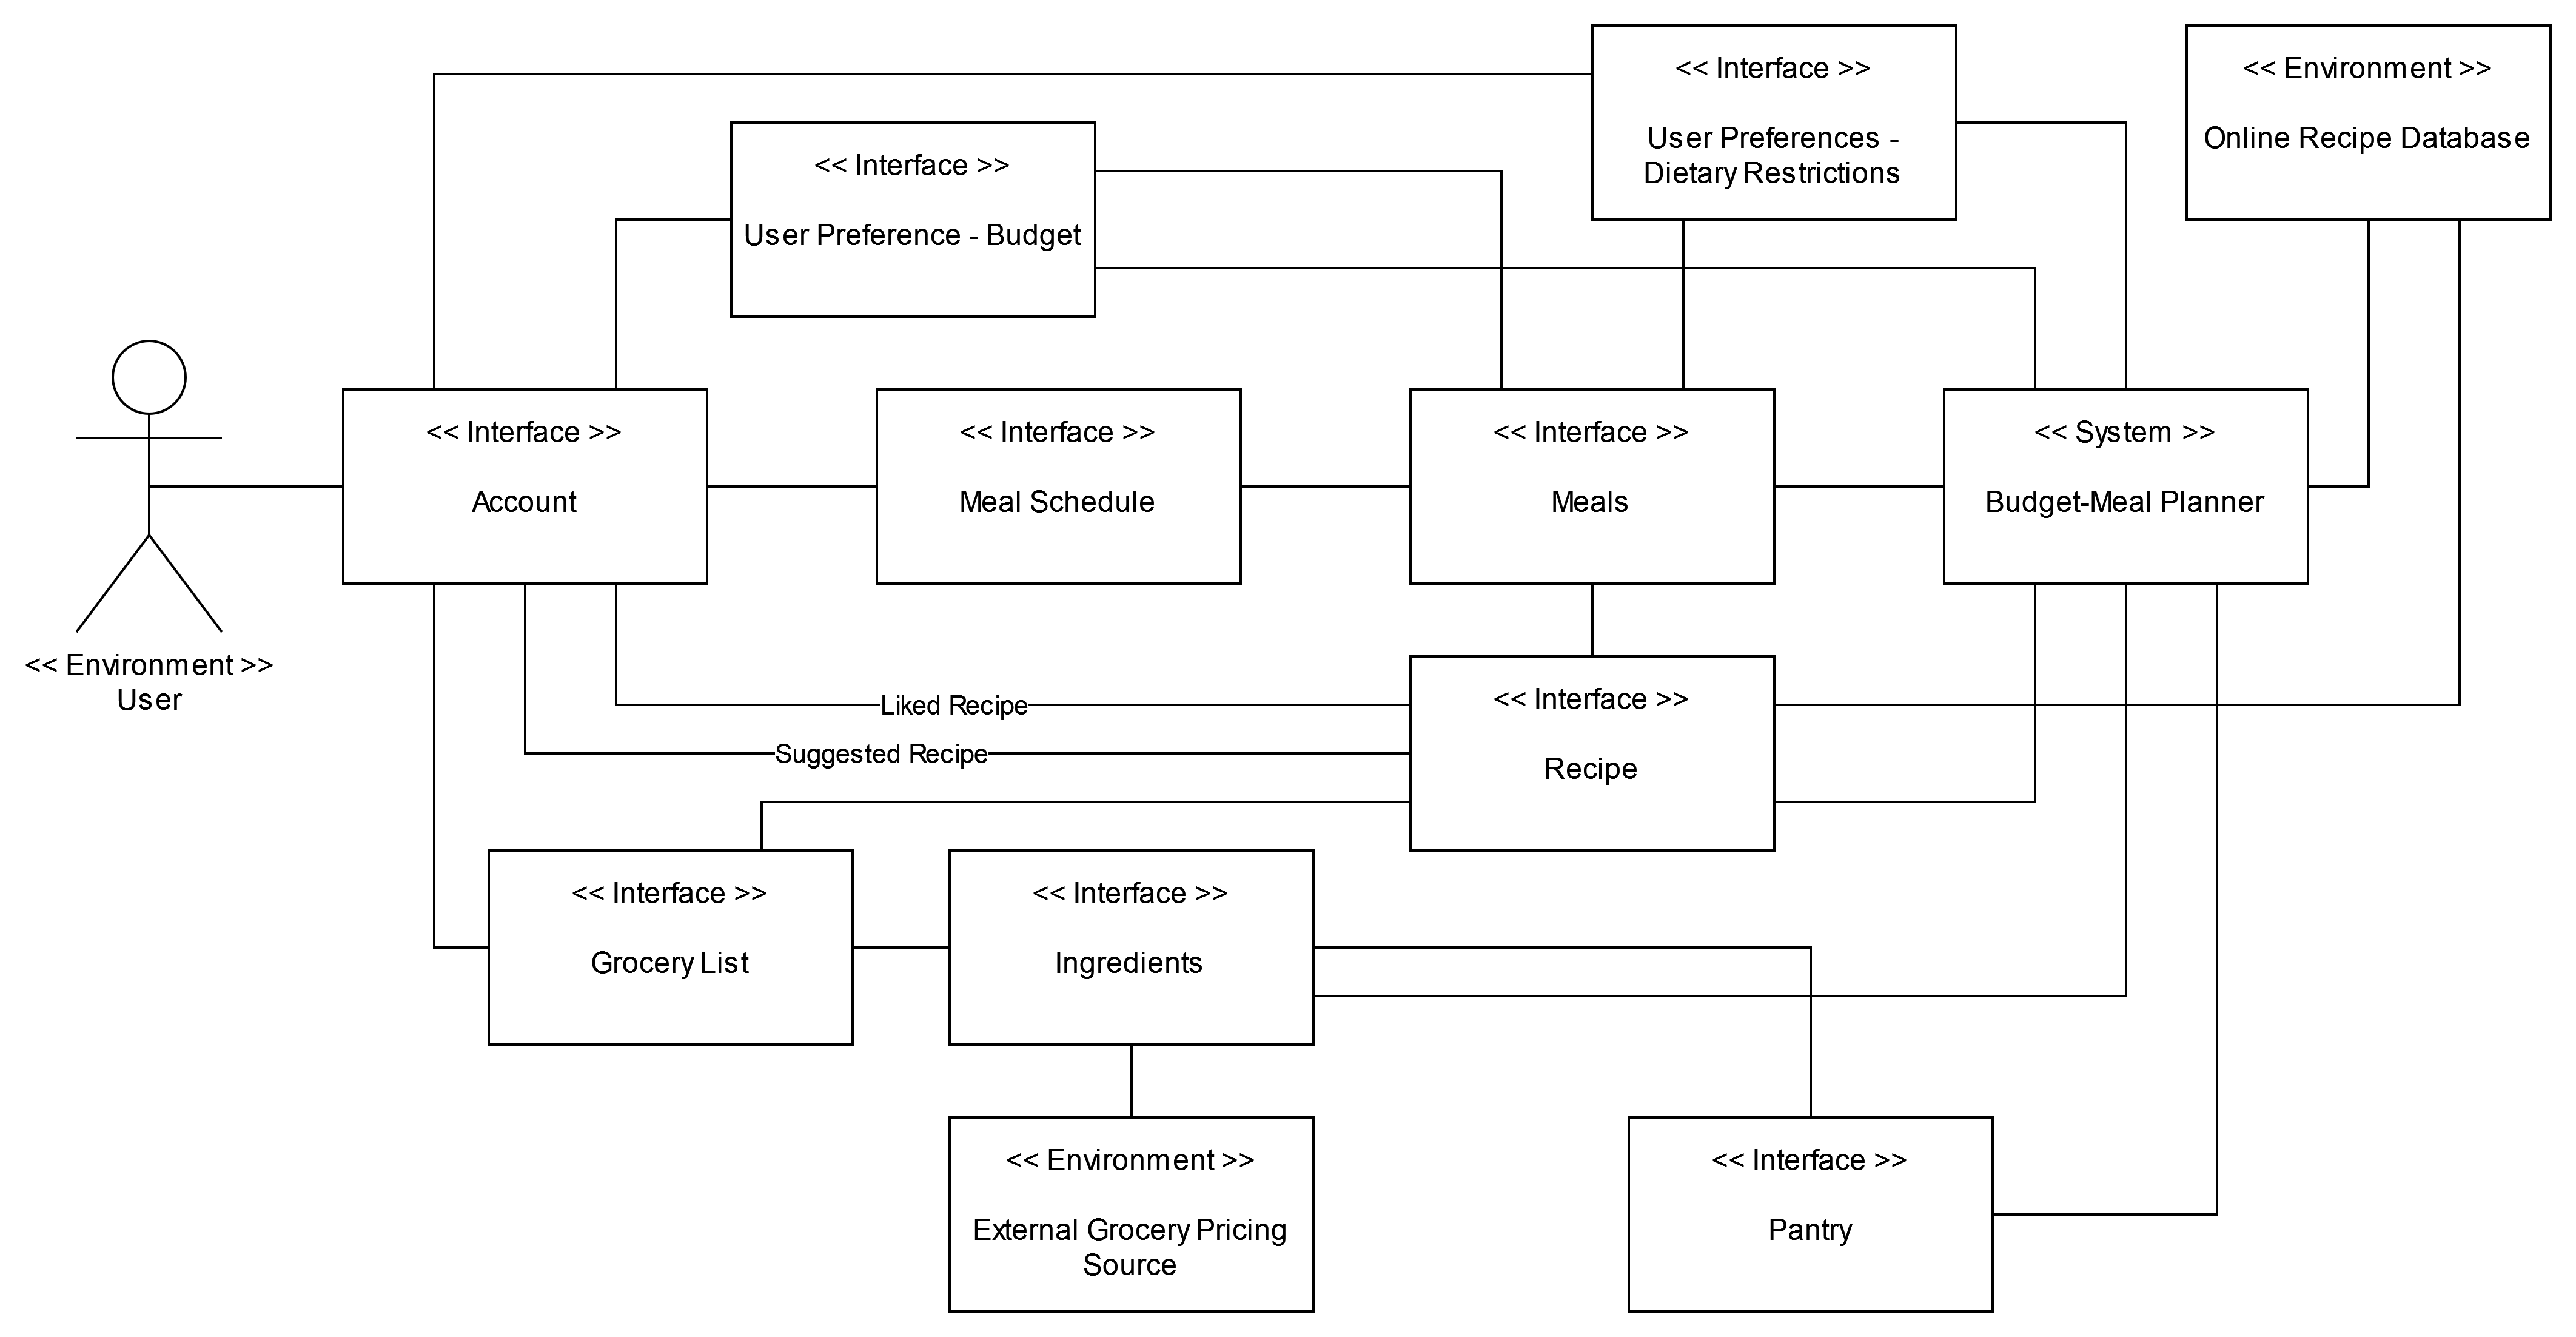
\includegraphics[width=\textwidth]{images/Domain_Model.png}
    \caption{Domain Model with World Diagram Superimposed}
\end{figure}

% Use Case Model
\chapter{Use Case Model}
\begin{figure}[h]
    \centering
    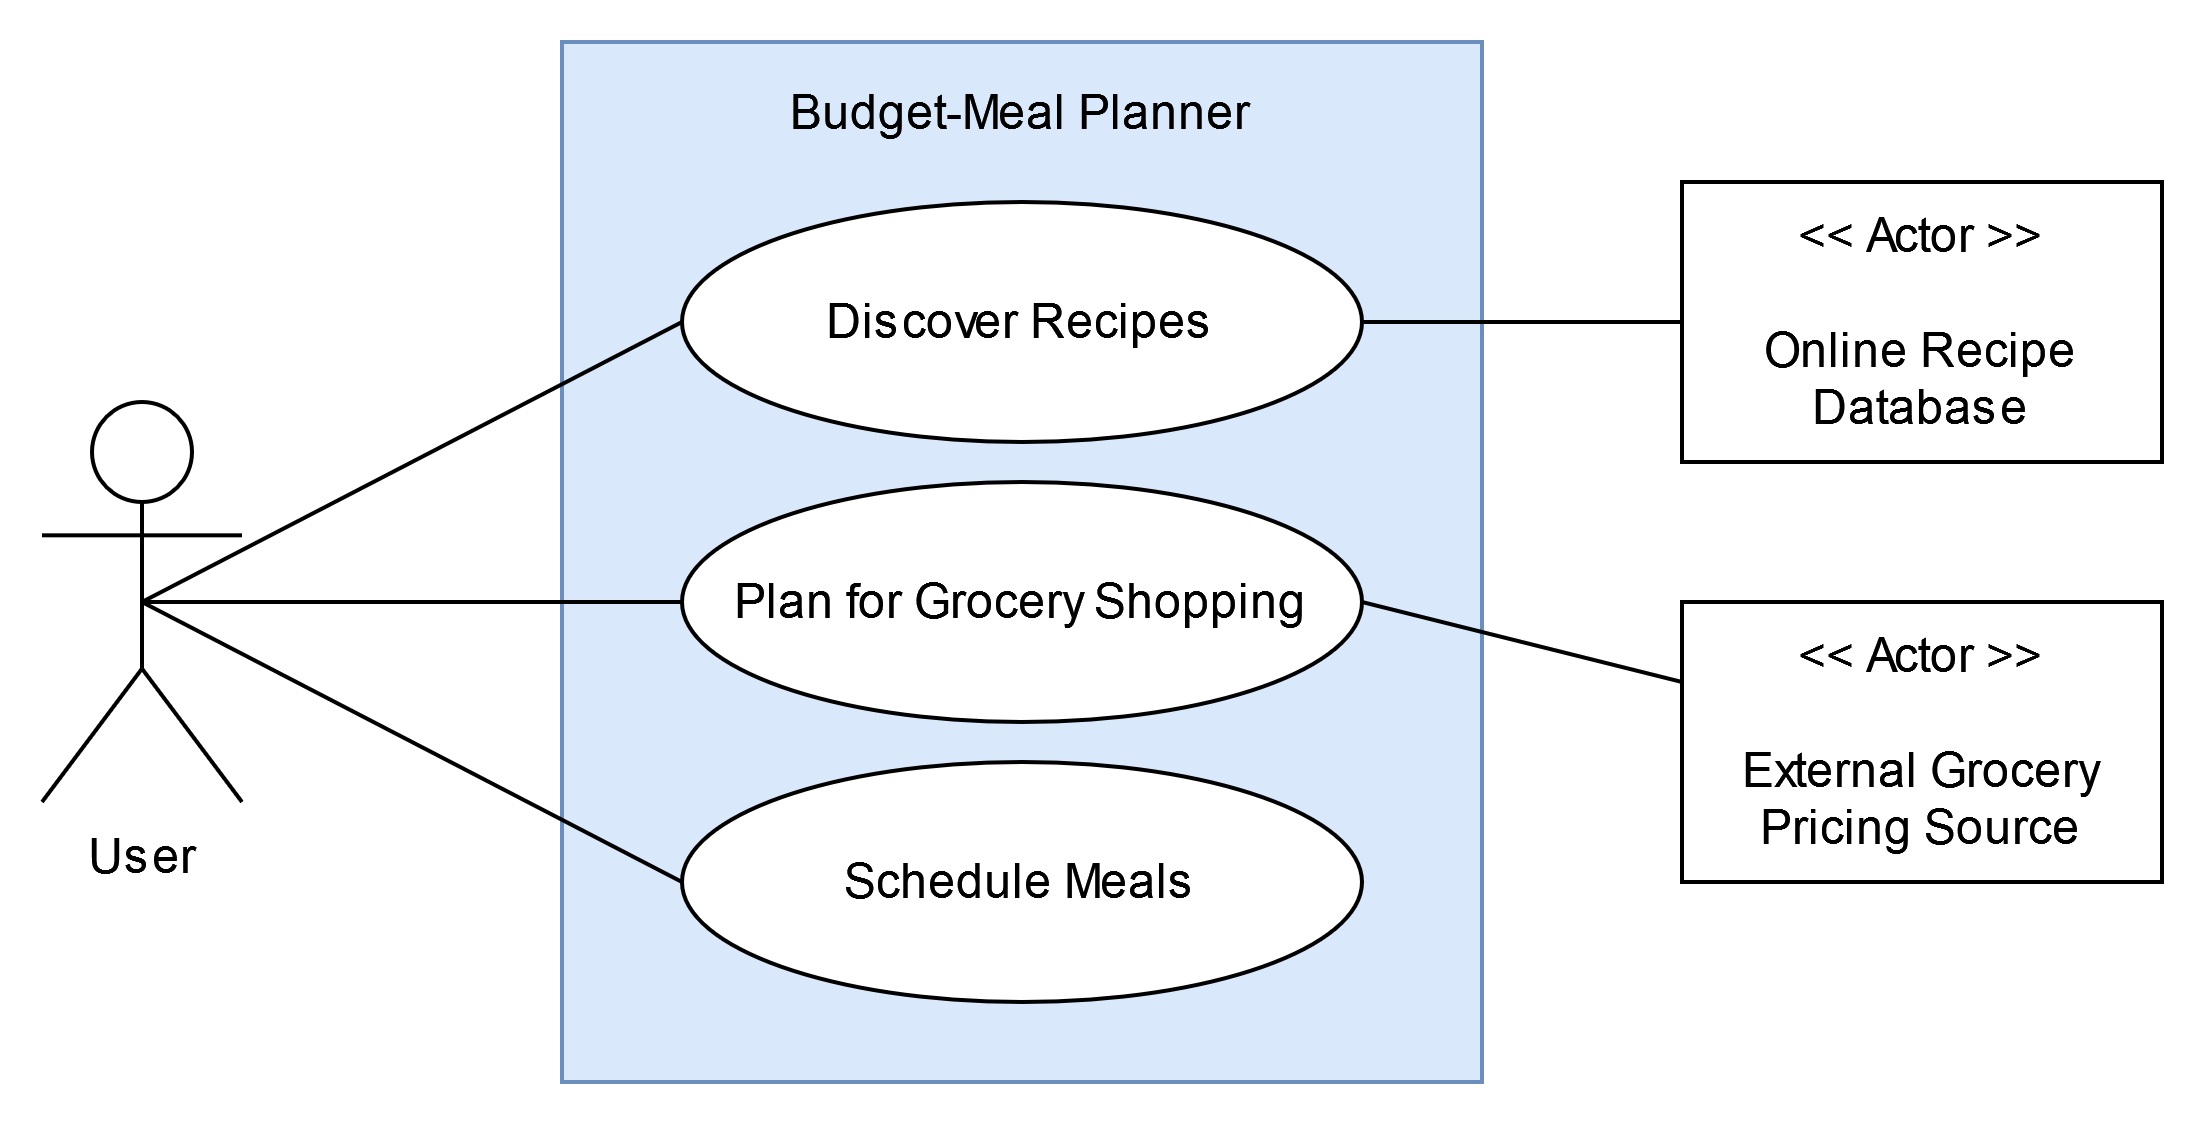
\includegraphics[width=\textwidth]{images/Use_Case.png}
    \caption{Use Case Model}
\end{figure}

\noindent \textbf{Discover Recipes}
\begin{itemize}
    \item Accept the users’ login credentials and open their account.
    \item Ask the user some questions to gather their preferences.
    \item Present the user with a list of recipes recommended for them.
    \item Accept a new recipe from the user and save it.
    \item Suggest alternative recipes, similar to the current recipe displayed.
    \item Hide a recipe from the user if they dislike it.
    \item Save a recipe to a “liked” collection for the user if they like it.
\end{itemize}
Domain Assumptions
\begin{itemize}
    \item The user has an account.
    \item Online Recipe Database is available.
    \item External Grocery Pricing Source is available.
    \item Recipe is valid, and can be cooked.
    \item The ingredients in the recipe are available in the External Grocery Pricing Source or the user’s pantry.
\end{itemize}

\noindent \textbf{Plan for Grocery Shopping}
\begin{itemize}
    \item Display the user’s current ingredient quantities in the pantry.
    \item Display the user’s grocery list.
    \item Add all ingredients from a recipe to the grocery list.
    \item Move ingredients from grocery list to pantry based on what the user bought from the grocery store.
\end{itemize}
Domain Assumptions
\begin{itemize}
    \item The user has an account.
    \item External Grocery Pricing Source is available.
    \item The currency of the External Grocery Pricing Source is the same as the user’s currency.
    \item The prices are up to date, and representative of the real world.
    \item 
\end{itemize}

\noindent \textbf{Schedule Meals}
\begin{itemize}
    \item Assign a recipe to a meal on a user’s schedule.
    \item Display a user’s meal plan (schedule).
\end{itemize}
Domain Assumptions
\begin{itemize}
    \item The user has an account.
    \item Recipes are accessible.
    \item There are enough recipes available to fill the user’s schedule.
    \item The ingredients for the meals are available in the user’s pantry, or can be procured.
\end{itemize}

% Scenarios
\chapter{Scenarios}
\noindent \textbf{UC 1: Discover Recipes} \\
% START UC 1 TABLES

\begin{xltabular}{\textwidth}{|X|X|X|}
\hline
User & Budget-Meal Planner & Online Recipe Database \\
\hline
1. Opens the Budget-Meal Planner &  &  \\
 & 2. Displays the login screen &  \\
3. Types in their username and password &  &  \\
 & 4. The user is logged in to the account with matching credentials &  \\
 & 5. The "Home" screen is displayed &  \\
6. Clicks the "Discover Recipes" button &  &  \\
 & 7. Displays a page with a search box at the top and a scrollable collection of the top 15 recipes related to the user's preferences, which have not been saved by the user &  \\
8. Clicks on a recipe &  &  \\
 & 9. Displays the recipe's details &  \\
10. Clicks the "Like" button &  &  \\
 & 11. Saves the recipe to the user's account, in the "Liked Recipes" section &  \\
12. Clicks the "Back" button &  &  \\
 & 13. Displays the collection of recipes again &  \\
14. Clicks the search box &  &  \\
 & 15. Displays a search bar with a "Search" button &  \\
16. Types in a search query &  &  \\
 & 17. Forwards the search query to the Online Recipe Database &  \\
 &  & 18. Returns a collection of recipes related to the search query \\
 & 19. Compares the collection of recipes returned by the online recipe database with the collection of recipes already saved to the user's account &  \\
 & 20. Removes any recipes already saved to the user's account from the collection and displays the remaining collection of recipes &  \\
21. Go To 8 &  &  \\
22. Clicks the "Home" button to return to the Home page &  &  \\
\hline
\end{xltabular}

\begin{xltabular}{\textwidth}{|X|X|X|}
\hline
\multicolumn{3}{|p{\dimexpr\linewidth-2\tabcolsep\relax}|}{Exception 1: The user enters an incorrect username or password} \\
\hline
User & Budget-Meal Planner & Online Recipe Database \\
\hline
 & E1.4. Checks the database for a matching username, if user does not exist, displays an error message, "Incorrect username or password. Try again." &  \\
E1.5. Go To 3 &  &  \\
 &  &  \\
\hline
\end{xltabular}

\begin{xltabular}{\textwidth}{|X|X|X|}
\hline
\multicolumn{3}{|p{\dimexpr\linewidth-2\tabcolsep\relax}|}{Exception 2: The online recipe database is unavailable} \\
\hline
User & Budget-Meal Planner & Online Recipe Database \\
\hline
 & E2.18. Attempts to connect to the online recipe database source &  \\
 &  & E2.19. No response or connection refused \\
 & E2.20. Retries the connection 3 times &  \\
 &  & E2.21. No response or connection refused after 3 retries \\
 & E2.22. Displays an error message, "Unable to retrieve search results. Please try again later." &  \\
E2.23. Acknowledges the error message &  &  \\
 & E2.24. Go To 7 &  \\
 &  &  \\
\hline
\end{xltabular}
% END UC 1 TABLES

\noindent \textbf{UC 2: Plan for Grocery Shopping} \\
% START UC 2 TABLES

\begin{xltabular}{\textwidth}{|X|X|X|}
\hline
User & Budget-Meal Planner & External Grocery Pricing Source \\
\hline
1. Clicks the "Grocery List" button &  &  \\
 & 2. Displays the user's empty grocery list with the message, "Add something to the list!", and a button to add ingredients &  \\
3. Clicks the "Add ingredients" button &  &  \\
 & 4. Displays a search bar and a list of common ingredients &  \\
5. Types in the search bar &  &  \\
 & 6. Displays a list of ingredients matching the search query &  \\
7. Clicks on an ingredient &  &  \\
 & 8. Displays a prompt, "How much {ingredient name} do you want to add?" and a number input field, along with the options "Yes" and "No" &  \\
9. Enters the quantity of the ingredient to add to the grocery list &  &  \\
 & 10. Updates the number input field with the quantity entered by the user &  \\
11. Clicks the "Yes" button &  &  \\
 & 12. Returns to the grocery list, with the ingredient added to the list with the quantity entered by the user &  \\
 & 13. Requests for the latest prices of ingredients in the grocery list from the external grocery pricing source. Rate limited to once per day. &  \\
 &  & 14. Returns the latest prices of ingredients in the grocery list \\
 & 15. Displays the user's grocery list with the latest prices &  \\
16. Clicks the checkbox next to the ingredient &  &  \\
 & 17. Displays a confirmation message, "Add ingredient to pantry?" with the options "Yes", "No", and "Modify Quantity" &  \\
18. Clicks the "Yes" button &  &  \\
 & 19. Moves the ingredient to the pantry, adds the quantity in the grocery list to what was already in the pantry &  \\
 & 20. Displays the user's pantry, containing a scrollable list of ingredients and their quantities &  \\
21. Clicks the "Home" button to return to the Home page &  &  \\
\hline
\end{xltabular}

\begin{xltabular}{\textwidth}{|X|X|X|}
\hline
\multicolumn{3}{|p{\dimexpr\linewidth-2\tabcolsep\relax}|}{Exception 1: The user's search query does not match any ingredients} \\
\hline
User & Budget-Meal Planner & External Grocery Pricing Source \\
\hline
 & E1.6. Displays a message, "No results found..." &  \\
E1.7. Go To 5 &  &  \\
 &  &  \\
\hline
\end{xltabular}

\begin{xltabular}{\textwidth}{|X|X|X|}
\hline
\multicolumn{3}{|p{\dimexpr\linewidth-2\tabcolsep\relax}|}{Exception 2: The external grocery pricing source is unavailable} \\
\hline
User & Budget-Meal Planner & External Grocery Pricing Source \\
\hline
 & E2.14. Attempts to connect to the external grocery pricing source &  \\
 &  & E2.15. No response or connection refused \\
 & E2.16. Retries the connection 3 times &  \\
 &  & E2.17. No response or connection refused after 3 retries \\
 & E2.18. Displays an error message, "Unable to retrieve latest prices. Please try again later." &  \\
E2.19. Acknowledges the error message &  &  \\
 & E2.20. Displays the user's grocery list with the latest prices from the last successful request &  \\
E2.21. Go To 5 &  &  \\
 &  &  \\
\hline
\end{xltabular}
% END UC 2 TABLES

\noindent \textbf{UC 3: Schedule Meals} \\
% START UC 3 TABLES

\begin{xltabular}{\textwidth}{|X|X|}
\hline
User & Budget-Meal Planner \\
\hline
1. Clicks the "Schedule" button &  \\
 & 2. Prompts the user with a message, "Schedule meals for the week?" \\
3. Clicks the "Yes" button &  \\
 & 4. Selects recipes from the app's local recipe database, and assigns them to every meal slot for the week \\
 & 5. Displays the user's weekly meal plan schedule \\
6. Clicks on a day of the week &  \\
 & 7. Displays the user's meal plan for that day \\
8. Clicks on a time slot for a meal &  \\
 & 9. Displays the meal details page \\
10. Clicks on a recipe &  \\
 & 11. Displays the recipe's details \\
12. Clicks the "Add ingredients to Grocery List" button &  \\
 & 13. Displays a confirmation message, "Add all ingredients to Grocery List?" with the options "Yes" and "No" \\
14. Clicks the "Yes" button &  \\
 & 15. Adds all ingredients in the recipe to the user's grocery list, adding quantities wherever possible \\
16. Clicks the "Home" button to return to the Home page &  \\
\hline
\end{xltabular}

\begin{xltabular}{\textwidth}{|X|X|}
\hline
\multicolumn{2}{|p{\dimexpr\linewidth-2\tabcolsep\relax}|}{Exception 1: The app is unable to find recipes for a meal slot} \\
\hline
User & Budget-Meal Planner \\
\hline
 & E1.4. Displays an error message, "Unable to find recipes to schedule. Please try again later." \\
E1.5. Acknowledges the error message &  \\
 & E1.6. Go To UC1.5 \\
 &  \\
\hline
\end{xltabular}

\begin{xltabular}{\textwidth}{|X|X|}
\hline
\multicolumn{2}{|p{\dimexpr\linewidth-2\tabcolsep\relax}|}{Exception 2: Fails to add ingredients to grocery list} \\
\hline
User & Budget-Meal Planner \\
\hline
 & E2.14. Displays an error message, "Unable to add ingredients to grocery list. Please try again." \\
E2.15. Acknowledges the error message &  \\
 & E2.16. Go To 11 \\
 &  \\
\hline
\end{xltabular}
% END UC 3 TABLES

% User Stories
\chapter{User Stories}
\end{document}
